% 编辑器使用说明
% keys 小时百科|在线编辑器|latex
% license CCBYSA3
% type Tutor

欢迎使用小时百科/云笔记编辑器。

该编辑器同时用于\href{https://wuli.wiki/editor/}{编辑小时百科}以及\href{https://wuli.wiki/note/}{小时云笔记}两个板块。 它们的功能几乎相同, 但百科有合作编辑功能而云笔记暂时没有。另外百科对文章的格式会有更多限制。
\begin{figure}[ht]
\centering
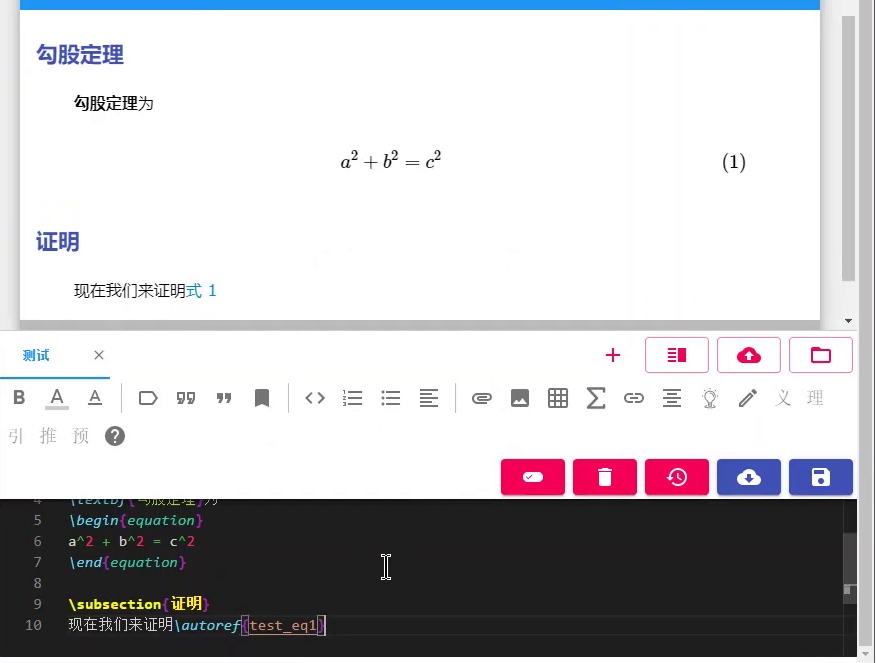
\includegraphics[width=13cm]{./figures/19c6cc6482ff004d.png}
\caption{编辑器截图(\href{https://wuli.wiki/apps/editor.gif}{查看 GIF 动画})} \label{fig_editor_3}
\end{figure}

\subsection{如果您已经会 LaTeX}
本编辑器只支持 LaTeX 的公式\footnote{公式渲染和知乎等网站一样使用\href{https://www.mathjax.org/}{MathJax}。 MathJax。}以及其他一些简单的 LaTeX 命令和百科自定义的命令(大部分可以通过菜单栏插入), 所以如果您\textbf{直接把别处的完整 LaTeX 代码复制进来几乎肯定会遇到严重的问题!编辑器仅支持百科的模板,请不要定义或修改任何模板设置!}

以下大部分不是 LaTeX 的教程而是编辑器的教程, 所以同样建议您看一看。 可能\textbf{大大提高编辑效率}的功能有: 引用按钮(自动添加 \verb|\label| 和 \verb|\autoref| 来引用公式图表等), 自动补全和符号替换(可以在设置里面自定义), 以及各种快捷键(\autoref{tab_editor_1})。

\subsection{视频教程}
\begin{itemize}
\item 编辑器零基础视频教程(\href{https://www.bilibili.com/video/av87698355/}{Biblibili}, \href{https://zhuanlan.zhihu.com/p/105869878}{知乎}, \href{https://www.youtube.com/watch?v=AN2tXNanD9U&t=1s}{YouTube})。
% \item \addTODO{提高编辑效率 (未完成): 使用代码补全, 符号显示, 自动引用, 实时预览, 符号显示。}
% \item \addTODO{其他功能(未完成): 编译 pdf, 转载到知乎等。}
\end{itemize}

\subsection{注册和申请}
要使用编辑器,您需要进行\href{https://wuli.wiki/forum}{注册}, 登录成功后, 要编辑百科访问 \href{https://wuli.wiki/editor/}{wuli.wiki/editor}, 云笔记则访问 \href{https://wuli.wiki/note/}{wuli.wiki/note}。
\begin{itemize}
\item \textbf{编辑百科:} 如果您只是进行一些细微的修改如错别字和笔误,则无需申请成为作者。 但如果您需要进行更多创作或修改, 则需要在\href{https://wuli.wiki}{网站主页}申请成为作者。 您的任何修改都需要我们在后台审核后方可生效(也可能不采用),这个过程一般需要少于一天。
\item \textbf{云笔记:}云笔记功能目前对所有注册用户开放,无需申请。 云笔记目前已经进入稳定阶段,数据会永久保留,定期备份,请放心使用。 注意我们会时常更新功能,可能偶尔会出现无法编辑,但不会丢失数据,一般数小时内会恢复正常。
\end{itemize}

\subsection{创作流程}
\subsubsection{新建或修改文章}
\begin{itemize}
\item 进入编辑器初始页面后, 点\textbf{新建文章}(红色加号)按钮可以新建文章(一个 \verb`tex` 文件), 点\textbf{打开文章}(红色文件夹)按钮可以编辑已有文章。
\item 新建的文章不会自动出现在\href{https://wuli.wiki/online/}{百科目录}中,需要手动编辑 \verb`main.tex` 以修改目录。
\end{itemize}

\subsubsection{发布}
\begin{itemize}
\item 申请成为百科作者后默认拥有新建和编辑普通文章和目录的权限, 但不能发布文章, 而是需要拥有 “\textbf{发布文章}” 权限的用户审核通过后发布。 没有发布的修改可以在 \href{http://wuli.wiki/changed/}{wuli.wiki/changed/} 中看到, 但无法在 \href{http://wuli.wiki/changed/}{wuli.wiki/online/} 或者 \href{http://wuli.wiki/book/}{wuli.wiki/book/} 中看到。
\item 用户对自己的云笔记具有一切权限,包括 “\textbf{发布文章}”。
\item 目前,百科管理员会每天对所有新建的和被修改的文章进行粗略的审核并发布(即使处于草稿阶段)。该审核主要是为了防止误删、恶意编辑和违规内容。更深入的内容讨论一般在创作群中,申请成为作者即可加入。
\end{itemize}

\subsubsection{占用}
\begin{itemize}
\item 若一篇文章被某个作者编辑, 则该文章被该作者\textbf{占用}。 其他用户无法修改该文章,只能以\textbf{只读模式}打开。
\item 有 “\textbf{占用管理}” 权限的用户可以解除占用,允许其他用户编辑。 当文章被发布时也会自动取消占用。
\item 目前,\textbf{总目录}(\verb`main.tex`)和\textbf{参考文献} (\verb`bibliography.tex`) 都会在最后一次编辑的 6 分钟后自动取消占用,无需管理帮助。
\end{itemize}

\subsection{LaTeX 结构}
一个简单的 LaTeX 介绍见 \href{https://wuli.wiki/online/latxIn.html}{LaTeX 结构简介}。 除公式外,绝大部分支持的命令都可以通过工具栏插入, 所有支持的命令见\enref{小时百科文章示例}{Sample}。

整个百科(或用户笔记)是 LaTeX 的一个 \verb|document| 环境, 主文件是 \verb|main.tex|(点击右上角的“打开文章”按钮,第一个就是), 目录中每个 “部分” 是一个 \verb|\part{}|, 每个 “章” 是一个 \verb|\chapter{}|, 每篇文章是一个 \verb|\section{}|, 文章中蓝色的小标题是 \verb|\subsection{}|, 黑色的小标题是 \verb|\subsubsection{}|。

每篇文章拥有独立文件 \verb|文章id.tex| 作为一个 \verb|\section{}| 插入 \verb|main.tex| 中。 这需要手动在 \verb|main.tex| 中使用百科自定义的 \verb|\entry{文章标题}{文章id}| 命令。 该命令相当于 \verb|\section{文章标题}\label{文章id}| 然后用 \verb|\input{文章id.tex}| 把文件内容直接插入到下方。

相比于传统的 LaTeX 编译器,我们对在线编辑器进行了一些优化,例如可以单独编译一篇文章而不是整个 \verb`main.tex`。线下编译百科的完整 pdf 通常需要 20 分钟以上。

网页版的百科文章目录由 \verb|main.tex| 文件生成, 所以必须把新建的文章在这里插入并保存才能更新目录。 否则虽然页面可以访问但却不会出现在目录中。

每篇文章文件(后缀名为 tex)都有一个独一无二的文件名(即 \verb`文章id`),限制为小于等于 6 个字母或数字,不区分大小写。可以将通过将光标停留在编辑器中的 tab 上查看或者通过地址栏的 url 查看。

\begin{figure}[ht]
\centering
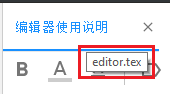
\includegraphics[width=4cm]{./figures/89cb63348bbde05a.png}
\caption{查看文件名(\verb`文章id`)} \label{fig_editor_2}
\end{figure}

每篇文章的 label 与文件名相同, 转换后输出的网页文件(html)也有相同的文件名, 可以在浏览器的地址栏中看到。例如本文的 LaTeX 文件是 \verb|EditRM.tex|, label 是 \verb|EditRM|, 网址(旧版界面)为 \href{https://wuli.wiki/online/EditRM.html}{wuli.wiki/online/EditRM.html}, 新界面的网址为 \href{https://wuli.wiki/EditRM}{wuli.wiki/EditRM}。

\subsection{公式}
\begin{itemize}
\item 公式环境支持大部分 LaTeX 命令, 严格来说是所有 \href{https://www.mathjax.org/}{MathJax} 支持的命令。
\item 我们在模板中用 \verb|\newcommand{}{}| 加入了一些自定义命令, 但不会覆盖原有的 LaTeX 命令。 若希望加入新的自定义命令, 请与管理员协商, 也可以使用下文的 “自动补全” 功能作为代替。
\item 一个简单的公式编辑器见\href{https://www.codecogs.com/latex/eqneditor.php}{这里} (不建议使用, 建议练习手动输入)。
\item 一个简单的 TeX/LaTeX 公式入门教程见\href{https://chaoli.club/index.php/211}{超理论坛}。
\item 本编辑器额外支持支持部分 \href{http://mirrors.ibiblio.org/CTAN/macros/latex/contrib/physics/physics.pdf}{Physics 宏包}中的命令,以及百科模板中自定义的快捷命令(见\enref{文章示例}{Sample})。
\item 行内公式插入到两个美元符号之间, 如 \verb|$a^2+b^2=c^2$| 显示为 $a^2 + b^2 = c^2$。
\item 独立公式只能用 \verb|equation| 环境(推荐), \verb|align| 环境或者 \verb|gather| 环境。 \verb|equation| 环境可以通过工具栏的公式图标插入, 也可以打 \verb|\beq| 然后按 Tab 键或者回车插入, 如
\begin{equation}\label{eq_editor_1}
a^2 + b^2 = c^2~,
\end{equation}
\item 公式中所有常用的和自定义的命令见\enref{文章示例}{Sample}。
\item 为增加代码可读性, 公式中一些命令会显示为对应的符号(如希腊字母, 求和符号, 不等号等), 注意这不会影响源码(复制时得到的也是命令而不是符号)。 设置面板(齿轮图标)可以选择关闭该功能。
\item 工具栏中的 “内部引用” 按钮可以引用同一页面的公式并生成链接(图片表格等同理), 如 “\autoref{eq_editor_1}”。 “外部引用” 按钮可以引用其他文章的公式或图表。
\end{itemize}

\subsection{菜单栏}
\begin{itemize}
\item 将光标停留在任意按钮上都会出现提示说明按钮的名称。 要新建文章, 点击红色的加号按钮, 根据提示新建即可。 要打开已有文章, 点击最右边的打开, 搜索需要的文章即可。
\item \textbf{加粗}、\textbf{斜体}、\textbf{大标题}、\textbf{小标题}按钮:可以在选中一段文字后按下,给这段文字添加相应格式。 也可以按下以后再填写需要的文字。
\item \textbf{预备知识}按钮,用于插入预备知识列表 \verb`\pentry{知识点1\nref{节点id1},知识点2\nref{节点id2}}{节点id}`。 具体用法详见\enref{小时百科文章示例}{Sample}。
\item \verb`\pentry{}{}` 中的 \verb`\nref{}` 链接可以通过 “外部引用”(空心双引号)按钮中的 “节点” 按钮来插入。 在提示 “输入序号” 时,如果不输入,则引用一篇文章的默认节点(即依赖于整篇文章)。 注意该命令暂时只能在 \verb`\pentry` 内部使用。
\item \textbf{内部引用}按钮(实心双引号图标)可以引用同一文章的公式, 图表, 例题,子节等。
\item \textbf{外部引用}按钮(空心双引号图标)可以引用其他文章的各种环境。 被引用对象没有 label 时会自动插入 label。
\item \textbf{引用文献}按钮(\textbf{[1]} 图标)可以引用\href{https://wuli.wiki/online/bibliography.html}{参考文献}(\verb`bibliography.tex`)并在文末列出。
\item \textbf{插入链接}按钮(回形针图标),可以给选中文字创建其他网站的链接,如\href{http://www.example.com}{链接文字}。 注意不能用于引用百科其他文章(要用 \verb`\enref{}`)。
\item \textbf{注释}按钮(\textbf{\%} 图标)可以把选中的文字注释或者取消注释。
\item \textbf{脚注}按钮,可以添加脚注,也支持把选中的一段文字变为脚注。
\item \textbf{窗口定位按钮}如果要在网页预览和 LaTex 代码之间跳转到对应位置, 可以通过搜索关键词实现。 例如在预览窗口复制一段文字, 在编辑窗口搜索就可以跳转到对应内容。(更新:现在可以直接选中后用 \verb`Alt` + \verb`F` 或者定位按钮)
\item \textbf{修改文章信息}按钮(红色的 🛈 图标)可以修改文章标题、协议等信息。 它们会注释在每个 tex 文件的开头,详见 \verb`Sample.tex`。
\item \textbf{历史版本}按钮(红色的时钟图标):编辑器会将有改动的文章每隔 5 分钟备份一次, 可以用查看历史版本,可以勾选其中两个进行对比,也可以点击其中一个进行恢复。
\item \textbf{下载源文件}(蓝色云朵箭头图标)按钮仅限在\href{http://wuli.wiki/note/}{小时云笔记}中使用。 点击菜单栏的 “下载” 按钮可以下载所有 tex 文件以及图片, 然后用 TeXlive 的 XeLaTeX 编译 \verb|main.tex| 即可(需要编译 2 到 4 次,取决于 pdf 的页数), 推荐使用 TeXlive 2019 或者更新版本。 在 Linux 环境中也可以直接用 \verb|make| 命令编译(会自动编译足够的次数)。
\item \textbf{导出 Markdown 文件(转载到知乎)}按钮:普通用户仅限在\href{http://wuli.wiki/note/}{小时云笔记}中使用(百科编辑器中只有管理员可用), 点击 “导出 Markdown 文件” 按钮生成与知乎兼容的 md 文件(矢量图和表格等暂不兼容), 在知乎的回答或文章编辑器中直接导入该文件即可。
\item \textbf{全文搜索}按钮(地球和放大镜图标) 用于搜索百科所有文章中的 LaTeX 代码。 输入关键词即可, 默认支持正则表达式, 区分大小写。 该功能是通过命令行的 \verb|git grep| 命令实现的, 具体命令为 \verb|git grep --no-index 用户输入|, 详细功能参考\href{https://git-scm.com/docs/git-grep}{官方文档}。
\end{itemize}

\subsubsection{图片和附件}
\begin{itemize}
\item \textbf{图片管理}按钮可以上传图片或管理已有图片,每张图片可以上传不同格式,也可以上传制作每张图片所需的源代码或其他文件以便以后编辑。
\item 除了使用按钮,也可以直接使用快捷键 \verb`Ctrl` + \verb`V` 从剪切板粘贴图片, 例如先使用操作系统自带的截图, 再在代码窗口按, 可以自动上传剪切板中的图片并创建图片环境。
% \item 【新】新增了实时预览功能, 即改变代码时预览自动更新。 该功能仍然有一些小 bug 待修复, 如果遇到问题可以在设置面板中关闭。 在非实时预览模式下, 编辑过程中用快捷键 \verb|Ctrl+S| 可以保存并刷新预览(建议经常刷新, 便于定位错误)。 也可以用工具栏的保存图标。
\end{itemize}

\subsection{其他功能}
\begin{table}[ht]
\centering
\caption{Windows 快捷键}\label{tab_editor_1}
\begin{tabular}{|c|c|c|c|}
\hline
保存文章 & \verb|Ctrl| + \verb|S| & 打开文章 & \verb|Ctrl| + \verb|O| \\
\hline
新建文章 & \verb|Ctrl| + \verb|Alt| + \verb|N| & 关闭文章 & \verb|Ctrl| + \verb|Alt| + \verb|W| \\
\hline
查找文本 & \verb|Ctrl| + \verb|F| & 替换文本 & \verb|Ctrl| + \verb|H| \\
\hline
增大字号 & \verb|Shift| + \verb|Alt| + \verb|+| & 减小字号 & \verb|Shift| + \verb|Alt| + \verb|-| \\
\hline
显示编辑器选项 & \verb|Ctrl| + \verb|Q| & 跳转到某行 & \verb|Ctrl| + \verb|G| \\
\hline
撤销 & \verb`Ctrl` + \verb`Z` & 重做 & \verb`Ctrl` + \verb`Y` \\
\hline
向左缩进 & \verb`Tab` 或 \verb|Ctrl| + \verb|[| & 向右缩进 & \verb`Tab` 或 \verb|Ctrl| + \verb|]| \\
\hline
关闭不保存 & \verb|Shift| + \verb|点击关闭| & 注释选中的行 & \verb`Ctrl` + \verb`K` 松开再按 \verb`C` \\
\hline
\end{tabular}
\end{table}

\begin{table}[ht]
\centering
\caption{Mac 快捷键}\label{tab_editor_2}
\begin{tabular}{|c|c|c|c|}
\hline
保存文章 & \verb|Cmd+S| & 打开文章 & \verb|Cmd+O| \\
\hline
新建文章 & \verb|Cmd+Opt+N| + \verb|Alt| + \verb|N| & 关闭文章 & \verb|Ctrl+Opt+W| \\
\hline
查找文本 & \verb|Cmd+F| & 替换文本 & \verb|Cmd+H| \\
\hline
增大字号 &  & 减小字号 & \\
\hline
显示编辑器选项 & \verb|Ctrl+Q| & 跳转到某行 & \verb|Ctrl+G| \\
\hline
向左缩进 & \verb|Cmd+ [| & 向右缩进 & \verb|Cmd+]| \\
\hline
关闭不保存 & \verb|Shift+点击关闭| &  &  \\
\hline
\end{tabular}
\end{table}

\begin{itemize}
\item 【新】快捷功能: 若剪切板有图片(例如截图以后), 在编辑器中直接用 \verb|Ctrl+V| 就可以上传该图片。
\item 正文中请使用中文标点, 编辑器会自动把空心句号替换为全角实心句号(如果您在使用笔记功能,可以选择在设置中关闭这个功)。
\item 双击文章的 tab 也可以关闭文章。
\item 任何时候打出反斜杠会自动提示可以自动补全的命令, 用上下键选择, 用 Tab 键或回车确认。 候选词未必是从最左边开始匹配, 例如打 \verb|\tbf| 按 tab 就会得到 \verb|\textbf{}|。
\item 如果自动补全带括号, 例如 \verb|\frac{}{}|, 补全后光标会自动进入第一个大括号, 再次按 Tab 光标会跳到第二个括号, 再按 Tab 光标会跳到第二个大括号外。
\item 打 \verb|\beq| 按 Tab 会自动出现 \verb|\begin{equation}...\end{equation}|, 其他环境也同理(\verb`itemize` 环境用 \verb`\bit`, \verb`enumerate` 环境用 \verb`benu` 等)。
\item 用光标选中一串字符后按下加粗按钮, 这串字符会自动插入 \verb|\textbf{}| 中。 同样, 选中字符串后输入 \verb|(| 等括号, 这个字符串会自动插入 \verb|()| 中。 表示行内公式的 \verb|$$| 也支持该操作。 用 “对齐” 按钮添加 \verb|aligned| 环境同理。
\item 编辑器在生成网页时会将编辑器中的 LaTex 代码转换为通用的 LaTex 代码(网页中右键点击公式获得), 即不需要自定义命令和额外宏包, 可以在任何支持 LaTeX 公式的环境使用(如知乎的公式编辑器)。
\item 编辑器支持一键转载到知乎(有少量不兼容, 例如表格和代码), 使用菜单栏的 “导出 Markdown 文件” 按钮, 然后将导出的文件上传到知乎即可。 该功能只能在编辑个人笔记时使用, 未经允许请勿转载百科内容。
\item 若要搜索整个百科的 LaTex 源码, 用\href{https://github.com/MacroUniverse/PhysWiki-log/tree/master/contents}{这个页面}, 若要搜索所有作者的编辑历史, 用\href{https://github.com/MacroUniverse/PhysWiki-backup}{这个页面}。
\end{itemize}

\subsection{设置面板}
编辑器中的 “设置” 按钮(齿轮图标)可以添加 “自动补全” 规则。 “自动补全” 如上文所描述的, 在输入 LaTeX 命令的过程中, 候选框会显示可以补全的命令, 用上下键选择命令, 然后用 tab 键或回车键补全。 补全规则的格式说明可以点击设置面板中的帮助按钮获得。

【已停用】 “符号替换” 功能是指, 在 LaTeX 公式中输入一些命令时, 编辑器会自动将其显示为对应的符号, 例如 \verb|\alpha| 显示为 \lstinline|α|, \verb|\sum| 显示为 \lstinline|∑| 等。 这样做是为了增加源码的可读性, 注意这只是一种视觉效果, 不会影响源码本身。 设置面板中的也可以添加 “符号替换” 规则或者将其关闭。

\addTODO{详细介绍设置面板的其他按钮}
\addTODO{tab 可以拖动}
